\section{Data and MC Performance}
\label{dataVsMc}
Given the limited number of recorded events passing the trigger and
vertex requirements, the collected statistics allow us to investigate
only the pixel barrel vlolume, that is the tracker region presently
giving the best performance in terms of conversion reconstruction.

A sample of conversions in this region is selected by applying the
following cuts designed to guarantee a good balance between purity and
efficiency:
\begin{itemize}
\item tracks with at least 4 hits;
\item track $d_0\cdot q > 0.1\cm$;
\item track pair opening angle on X-Y plane $\Delta\phi<0.2$;
\item reconstructed conversion vertex radius $r<15\cm$;
\item reconstructed conversion vertex longitudinal position $|z|< 26\cm$;
\item reconstructed transverse momentum of the converted photon $p_T<5\GeV$.
\end{itemize}

Expected performance in terms of efficiency and purity have been
estimated on the MC sample.
Efficiency is defined as the number of associated conversions
$N^{\rm assoc}_{\gamma}$ divided by the total number of simulated
conversions $N^{\rm sim}_{\gamma}$, while purity is defined as
$N^{\rm assoc}_{\gamma}$ divided by the number of reconstructed
conversions $N^{\rm reco}_{\gamma}$.
A reconstructed conversion is considered associated if simulated and reconstructed vertex positions match within a $10\times10\times10\cm^3$ 
box\footnote{A more proper association criteria, based on the hit
  association of the electron tracks, cannot be applied on the used MC
  sample. However, it was proven that the hit and vertex position
  association methods provide compatible results}.
Figure~\ref{efficpurity} shows that performance degrade for radius greater than $5\cm$, i.e. outside the first pixel barrel layer.
Very likely the main reason for this effect is the current tracking configuration, allowing for the reconstruction of very low $p_T$ tracks from
pixel hit-triplets only. A different tune of $p_T$ thresholds in iterative tracking steps could improve performance at larger radii.
%efficiency
%purity
\begin{figure}[!hbtp]
\subfigure[]{
\centering
\label{efficpurity_vs_r}
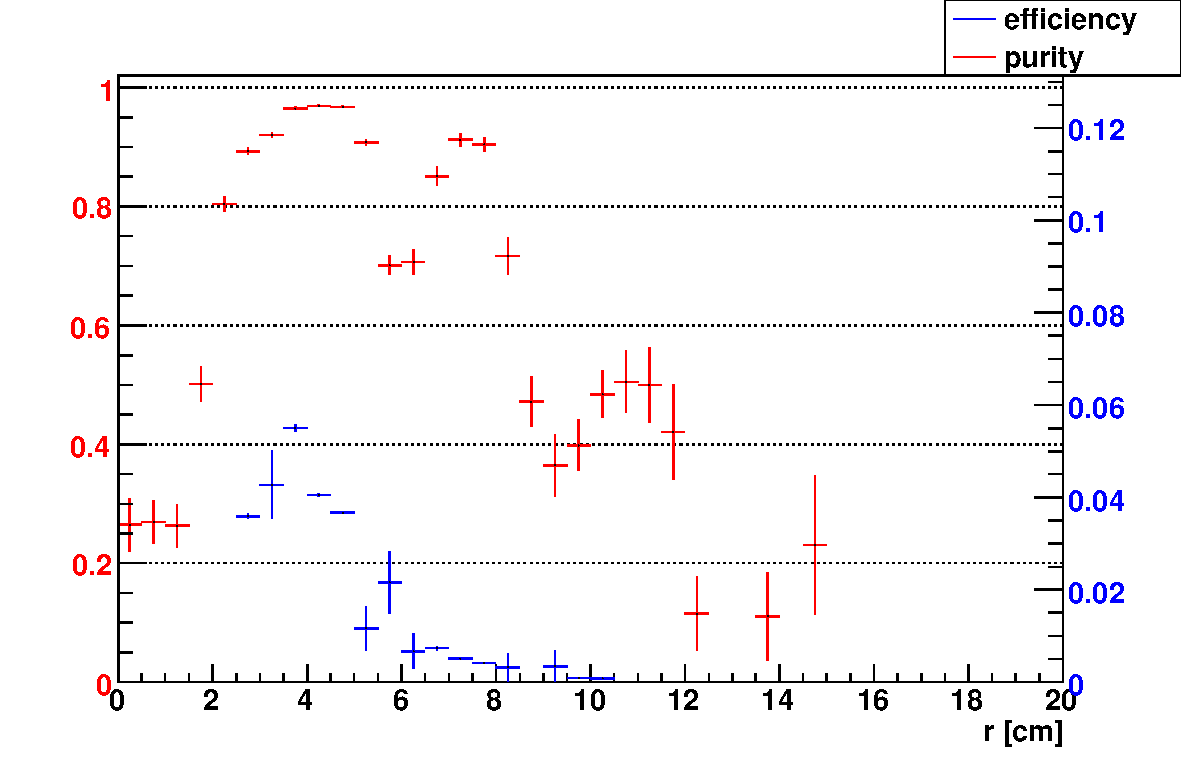
\includegraphics[width=.45\textwidth]{efficpurity_vs_r.pdf}}
\subfigure[]{
\centering
\label{efficpurity_vs_pt}
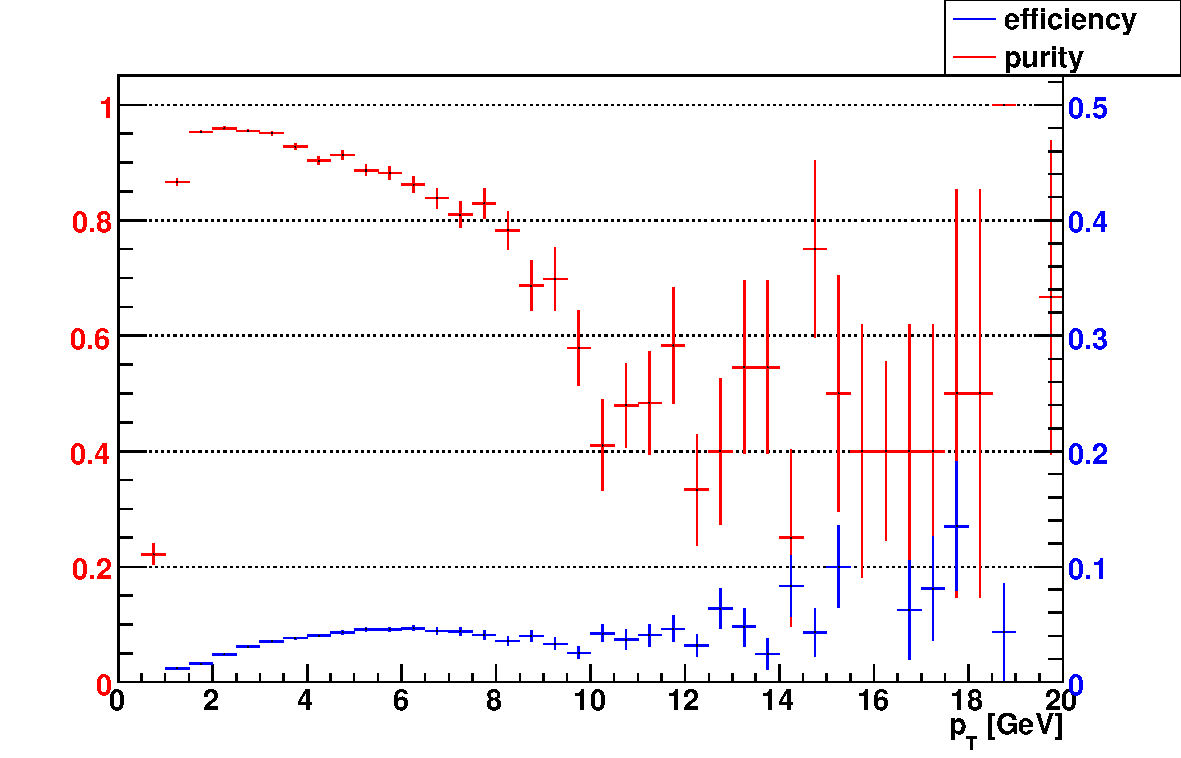
\includegraphics[width=.45\textwidth]{efficpurity_vs_pt.pdf}}
\caption{Efficiency (blue) and purity (red) vs $r$\subref{efficpurity_vs_r} and $p_T$\subref{efficpurity_vs_pt}.}
\label{efficpurity}
\end{figure}

In order to check that the conversion algorithm is providing
reasonable results with collision data, the basic conversion
distributions are compared to what is expected form MC. Converted
photon $p_T$, $\eta$ and $r$ are reported in
Figures~\ref{fig:eta}-\ref{fig:r}. Shapes show a nice agreement
between data and MC, while the number of comversions (normalized to
the total number of events) is $\sim10\%$ higher in data with respect
to MC. Such discrepancy could be due to several effects, like a higher
number of fakes in data or differences in the MC photon flux
and it is acceptable for the sake of the present preliminary study.
\begin{figure}[!hbtp]
\centering
\subfigure[]{
\label{subfig:eta_lin}
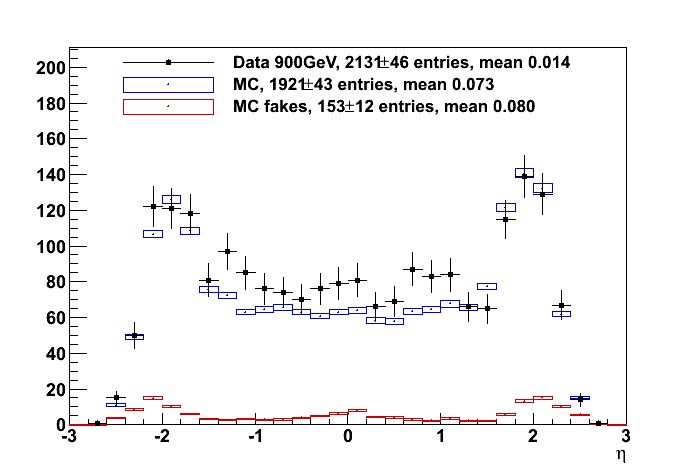
\includegraphics[width=.45\textwidth]{eta_lin.png}}
\subfigure[]{
\label{subfig:eta_log}
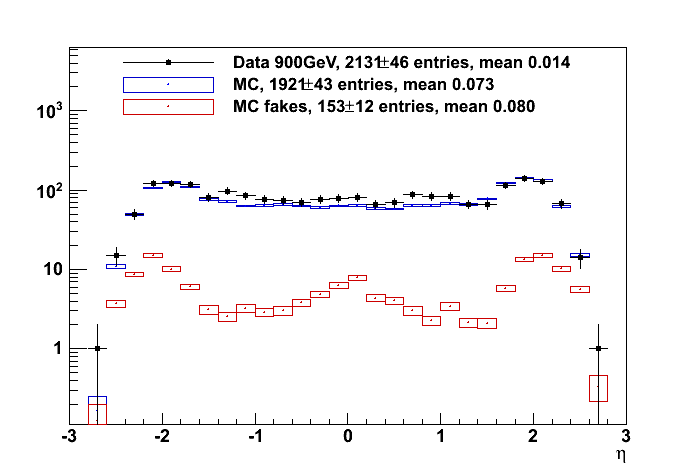
\includegraphics[width=.45\textwidth]{eta_log.png}}
\caption{Eta distribution of reconstructed conversions in linear\subref{subfig:eta_lin} and logaritmic\subref{subfig:eta_log} scale.
Data is shown in black dots and MC in blue boxes. Red boxes represent the expected fake contribution.}
\label{fig:eta}
\end{figure}

\begin{figure}[!hbtp]
\centering
\subfigure[]{
\label{subfig:pt_lin}
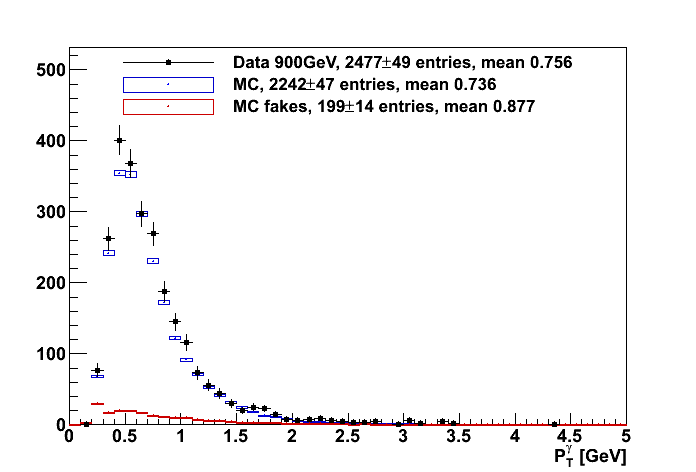
\includegraphics[width=.45\textwidth]{pt_lin.png}}
\subfigure[]{
\label{subfig:pt_log}
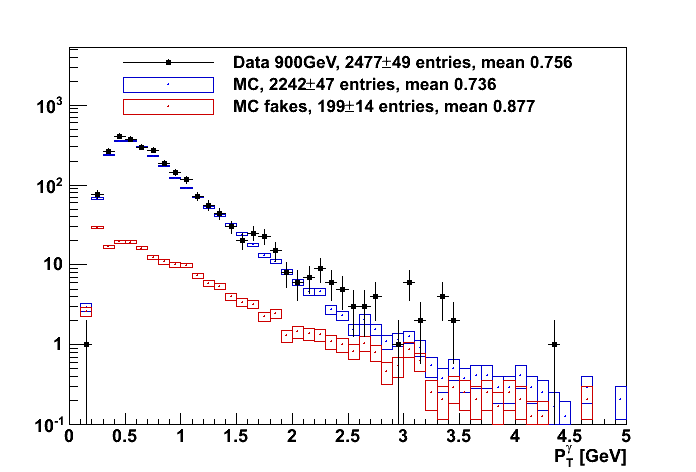
\includegraphics[width=.45\textwidth]{pt_log.png}}
\caption{$p_T$ distribution of reconstructed conversions in linear\subref{subfig:pt_lin} and logaritmic\subref{subfig:pt_log} scale.
Data is shown in black dots and MC in blue boxes. Red boxes represent the expected fake contribution.}
\label{fig:pt}
\end{figure}

\begin{figure}[!hbtp]
\centering
\subfigure[]{
\label{subfig:r_lin}
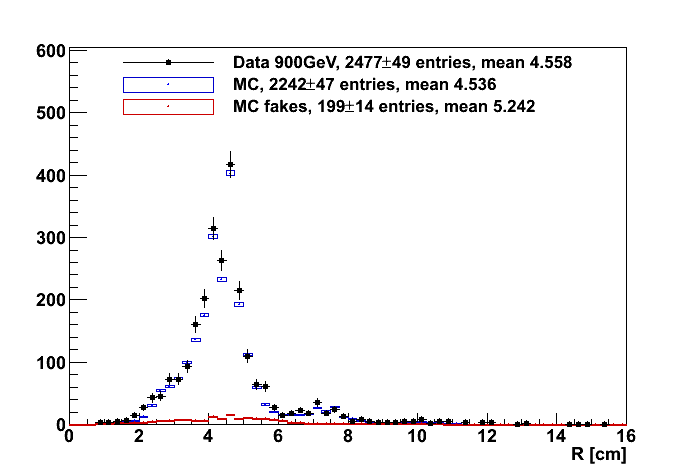
\includegraphics[width=.45\textwidth]{r_lin.png}}
\subfigure[]{
\label{subfig:r_log}
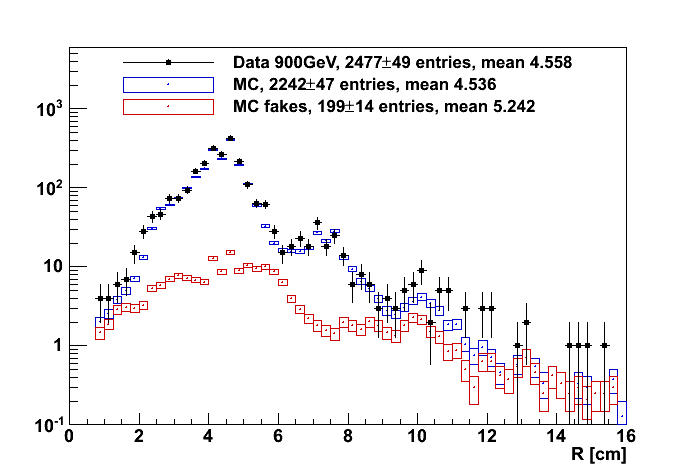
\includegraphics[width=.45\textwidth]{r_log.png}}
\caption{Radius distribution of reconstructed conversions in linear\subref{subfig:r_lin} and logaritmic\subref{subfig:r_log} scale.
Data is shown in black dots and MC in blue boxes. Red boxes represent the expected fake contribution.}
\label{fig:r}
\end{figure}
